% Licensed to the Apache Software Foundation (ASF) under one or more
% contributor license agreements. See the NOTICE file distributed with
% this work for additional information regarding copyright ownership.
% The ASF licenses this file to You under the Apache License, Version 2.0
% (the ``License''); you may not use this file except in compliance with
% the License. You may obtain a copy of the License at
%
% http://www.apache.org/licenses/LICENSE-2.0
%
% Unless required by applicable law or agreed to in writing, software
% distributed under the License is distributed on an ``AS IS'' BASIS,
% WITHOUT WARRANTIES OR CONDITIONS OF ANY KIND, either express or implied.
% See the License for the specific language governing permissions and
% limitations under the License.

\begin{changemargin}{1.5in}{0in}

\section{Overview}

The MetaCarta GTS appliance indexes documents and allows users to search
these documents based on both keywords and geographic references. The
MetaCarta Documentum Connector allows system administrators to configure
connections to Documentum repositories and define jobs to maintain
synchronization between the repositories and the GTS index.

This document specifies the means for connecting to these repositories,
indexing files from these repositories, and maintaining connections to
these repositories.

\subsection{Assumptions}

This document assumes you have a basic level of familiarity with GTS
appliance administration. This document also assumes that you have
a basic understanding of the repositories to which you are trying to
connect. If you need more information about the MetaCarta GTS appliance,
please read the \documentref{MetaCarta GTS Administrator's Guide} stored
on the appliance at \dirpath{/usr/share/doc/metacarta/AdminGuide.pdf}. For
more information about Documentum, please see your Documentum documentation
or Documentum administrator.

Throughout this document, we assume that your appliance is named \\
\url{metacarta.example.com}. 


%What is the name of the product package? I am just calling it
% Connector Addon for now.

\section{Installation}

The Documentum Connector is included with the Connector Addon
available from Metacarta. % Licensed to the Apache Software Foundation (ASF) under one or more
% contributor license agreements. See the NOTICE file distributed with
% this work for additional information regarding copyright ownership.
% The ASF licenses this file to You under the Apache License, Version 2.0
% (the ``License''); you may not use this file except in compliance with
% the License. You may obtain a copy of the License at
%
% http://www.apache.org/licenses/LICENSE-2.0
%
% Unless required by applicable law or agreed to in writing, software
% distributed under the License is distributed on an ``AS IS'' BASIS,
% WITHOUT WARRANTIES OR CONDITIONS OF ANY KIND, either express or implied.
% See the License for the specific language governing permissions and
% limitations under the License.

If you have not already installed the Connector Addon, you should use
the Connector Addon DVD to install it using the following steps:

\begin{enumerate}

\item Insert the DVD in your appliance.

\item Install the Connector Addon:

\begin{console}

metacarta:\~{}\$ sudo upgrade\_control install --from-dvd 

\end{console}

This will restart your appliance and eject the Connector Addon DVD.

\item Upgrade your license file, if necessary. For instructions,
see the \documentref{MetaCarta Appliance Administrator's Guide} or 
contact Customer Support (see page \pageref{SupportContact}).

\end{enumerate}

The Connector Addon cannot be uninstalled.

\subsection{Remote Updates}

In some cases, it may be very difficult to get physical access to an
appliance in order to install new software. To make the installation
process easier, MetaCarta provides a mechanism for remote
installations.  MetaCarta will provide you with ISO images of the
software you need upon request.  In brief, you can install the 
Connector Addon from ISO with the following command:

\begin{console}

metacarta:\~{}\$ sudo upgrade\_control install /path/to/iso.iso

\end{console}

For more information on the use of ISO
images for remote installations, see the \documentref{MetaCarta GTS
Administrator's Guide} stored on the appliance at
\dirpath{/usr/share/doc/metacarta/AdminGuide.pdf}.


\section{Configuration}

\subsection{Access to the Connector}

The administrator to the Documentum Connector % Licensed to the Apache Software Foundation (ASF) under one or more
% contributor license agreements. See the NOTICE file distributed with
% this work for additional information regarding copyright ownership.
% The ASF licenses this file to You under the Apache License, Version 2.0
% (the ``License''); you may not use this file except in compliance with
% the License. You may obtain a copy of the License at
%
% http://www.apache.org/licenses/LICENSE-2.0
%
% Unless required by applicable law or agreed to in writing, software
% distributed under the License is distributed on an ``AS IS'' BASIS,
% WITHOUT WARRANTIES OR CONDITIONS OF ANY KIND, either express or implied.
% See the License for the specific language governing permissions and
% limitations under the License.

must have
access to the web interface at
\url{http://metacarta.example.com/crawler/}. In the default appliance
security setup, you must have a Basic Authentication account
configured for access to the Connector web interface at
\url{http://metacarta.example.com/crawler/}.  If you are not an appliance
administrator, please ask the appliance administrator to give you such
an account.

An appliance administrator can create an account with access to the
ingestion interface (in this case, username {\tt fred} and password
{\tt ginger}) by running the following command on the appliance:

\begin{console}
metacarta:\~{}\$ basic\_auth\_control add ingest\_users fred:ginger 
\end{console}

Depending on how you have configured authentication using the
\command{auth\_control} tool, you may need to make changes other than
adding yourself to the ingest\_users group. For more information on
security configuration and \command{auth\_control}, see the Security
Administration section of the \documentref{MetaCarta Appliance
Administrator's Guide}.


\subsection{Initial Documentum Setup}

% Licensed to the Apache Software Foundation (ASF) under one or more
% contributor license agreements. See the NOTICE file distributed with
% this work for additional information regarding copyright ownership.
% The ASF licenses this file to You under the Apache License, Version 2.0
% (the ``License''); you may not use this file except in compliance with
% the License. You may obtain a copy of the License at
%
% http://www.apache.org/licenses/LICENSE-2.0
%
% Unless required by applicable law or agreed to in writing, software
% distributed under the License is distributed on an ``AS IS'' BASIS,
% WITHOUT WARRANTIES OR CONDITIONS OF ANY KIND, either express or implied.
% See the License for the specific language governing permissions and
% limitations under the License.

The Documentum connector uses a special configuration file located at
\dirpath{/etc/documentum.dmcl.ini} on the GTS appliance.  In many cases,
it will be possible to simply copy the \dirpath{dmcl.ini} file from an
appropriate Webtop server onto your appliance. The appliance uses DFC
version 5.3.5; if the Webtop server uses a different version, this may not
work. In any case, the configuration file may need additonal editing. For
example, you may need to alter your configuration file if your server uses
special routing or security features. Changing your configuration may also
help if the appliance is having trouble connecting or performance is poor.

If you need to make changes, ask your Documentum administrator for
assistance with editing the configuration file.  The configuration of
the GTS appliance should be similar to that of other devices, such as
Webtop servers, that connect directly to the Documentum server.

If you do not have access to the \dirpath{dmcl.ini} file from a
Webtop server, you can configure the Documentum connector from
the appliance command line with sudo access. (If you do not have
sufficient access privileges to run this command, contact your
appliance administrator.)  First, you need to find out the hostname or
IP address of the Documentum server, or ``docbroker'', to which you will
connect. In this document, your Documentum server will be assumed to be
\url{dctmsrvr.example.com}. You will also need to know the connection
port for the Documentum server. From the appliance command line, you
should run:

\begin{consolewide}
metacarta:\~{}\$ sudo metacarta-setupdocumentum dctmsrvr.example.com port
\end{consolewide}

If your Documentum docbroker uses the default connection port 1489,
you do not need to include the optional \field{port} argument.


% Licensed to the Apache Software Foundation (ASF) under one or more
% contributor license agreements. See the NOTICE file distributed with
% this work for additional information regarding copyright ownership.
% The ASF licenses this file to You under the Apache License, Version 2.0
% (the ``License''); you may not use this file except in compliance with
% the License. You may obtain a copy of the License at
%
% http://www.apache.org/licenses/LICENSE-2.0
%
% Unless required by applicable law or agreed to in writing, software
% distributed under the License is distributed on an ``AS IS'' BASIS,
% WITHOUT WARRANTIES OR CONDITIONS OF ANY KIND, either express or implied.
% See the License for the specific language governing permissions and
% limitations under the License.

If you want to enforce Active Directory security on documents crawled
from \ifDocumentumGuide Documentum,\fi \ifLivelinkGuide Livelink,\fi
\ifShareGuide your network share,\fi \ifCombinedConnectorGuide your
repositories,\fi you must configure your appliance for Active
Directory support. Ask your administrator whether or not your
appliance is configured to use Active Directory.

For more information on this step, please see the \documentref{MetaCarta
GTS Administrator's Guide}, located on the appliance at
\dirpath{/usr/share/doc/metacarta}\linebreak\dirpath{
/AdminGuide.pdf}.


\section{Collecting Documents From Repositories} % Retitle this, yo.

The Connector Framework manages retrieving documents from different
repositories through \emph{jobs}. Jobs can be scheduled to run
regularly; each job connects to a single repository using a particular
set of credentials. Each job is tied to a \emph{repository
connection}. Repository connections contain information allowing the
connector framework to connect to a given repository --- that is, a
single instance of Documentum. Each repository connection is also tied
to an \emph{authority connection}. These authority connections manage
document security, making sure that when files have been indexed on
your GTS appliance, only authorized users are able to view them as
search results. Before you can create a job, you must create a
repository connection for the job to use. Each repository connection
should be set up with an appropriate authority, in this case a
Documentum authority connection. 

\subsection{Creating Authority Connections}

To create an authority connection, first go to the
main Connector Framework Administration interface at
\url{metacarta.example.com/crawler/}.  By default, your username and
password are the Ingestion Basic Auth username and password defined
earlier. 

You will see a sidebar like the one to the left. Click on ``List
Authority Connections'' and then you will be presented with the
list of authority connections. Click ``Add a new connection.''
You will see the following:

% Licensed to the Apache Software Foundation (ASF) under one or more
% contributor license agreements. See the NOTICE file distributed with
% this work for additional information regarding copyright ownership.
% The ASF licenses this file to You under the Apache License, Version 2.0
% (the ``License''); you may not use this file except in compliance with
% the License. You may obtain a copy of the License at
%
% http://www.apache.org/licenses/LICENSE-2.0
%
% Unless required by applicable law or agreed to in writing, software
% distributed under the License is distributed on an ``AS IS'' BASIS,
% WITHOUT WARRANTIES OR CONDITIONS OF ANY KIND, either express or implied.
% See the License for the specific language governing permissions and
% limitations under the License.

\begin{picture}(1,1)
  \put(-100,15){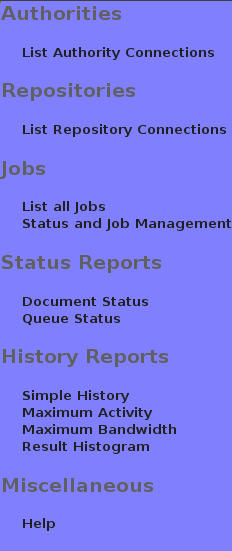
\includegraphics[width=80pt]{crawler-sidebar}}
\end{picture}


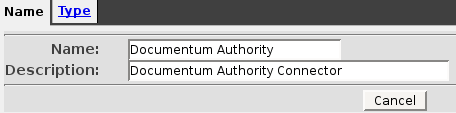
\includegraphics[width=300pt]{Docu-edit-authority-tab1}

This is the first tab of the tabbed interface you will use to edit
authority connections. The next tab is as follows:

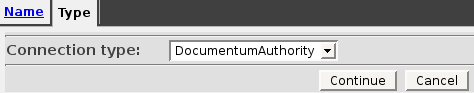
\includegraphics[width=300pt]{Docu-edit-authority-tab2}

In the first two tabs you must provide a name, description, and
authority type for your new authority connection. The name should be
unique, as you will use it to select this connection later when making
repository connections. The description should explain the authority
connection to you or another administrator. The authority type is the
type of authority to which you will connect, in this case a Documentum
Connection.

Once you have filled in those tabs, click continue, and then you must
fill in the following extra tabs specific to Documentum Authority
Connections:

% Licensed to the Apache Software Foundation (ASF) under one or more
% contributor license agreements. See the NOTICE file distributed with
% this work for additional information regarding copyright ownership.
% The ASF licenses this file to You under the Apache License, Version 2.0
% (the ``License''); you may not use this file except in compliance with
% the License. You may obtain a copy of the License at
%
% http://www.apache.org/licenses/LICENSE-2.0
%
% Unless required by applicable law or agreed to in writing, software
% distributed under the License is distributed on an ``AS IS'' BASIS,
% WITHOUT WARRANTIES OR CONDITIONS OF ANY KIND, either express or implied.
% See the License for the specific language governing permissions and
% limitations under the License.

\subsubsection{Configuring a Documentum Authority Connection}

The following options apply specifically to a Documentum authority
connector.  A Documentum authority connector manages document security
to a repository in conjunction with the Documentum server (or
``docbroker'') specified in the GTS appliance configuration.  Each
Documentum authority connector connects to only one Documentum
repository (or ``docbase''). If the docbroker used by the GTS
appliance has access to more than one docbase, you will need to create
an authority connector for each repository you wish to crawl.

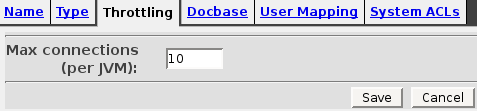
\includegraphics[width=300pt]{Docu-edit-authority-tab3}

\begin{itemize}

\item \textbf{Max Connections (per JVM):} The maximum number of
connections per JVM is important for two reasons.
\ifCombinedConnectorGuide \label{max-auth}\fi First, the number of
connections may impact the licensing on your document server,
depending on the repository. If you have a finite number of Documentum
connections available, they will be split between the authority
connector, which authorizes user access to documents, and the
repository connector, which actually downloads the documents to the
appliance. A default Documentum installation will have 100 connections
available; your Documentum installation may have more or less. It may
be advisable to lower the number of connections available to the
authority connector from the default value of 10. Ask your Documentum
administrator how many connections are available for use on your
Documentum system.

Second, the number of connections may impact the resources available
on the appliance. If the connector framework is slowing down your
appliance, lowering this number should help.

\end{itemize}

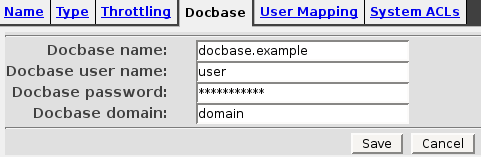
\includegraphics[width=300pt]{Docu-edit-authority-tab4}

\begin{itemize}

\item \textbf{Docbase name:} The host name of the Documentum
repository (or ``docbase'') with which you wish to connect.

\item \textbf{Docbase user name:} The user name that the GTS appliance
will use to connect to the docbase for this authority connection.
Typically, your Documentum administrator will create this account
specifically for use by the appliance. The account used by the GTS
appliance must have sufficient authority to retrieve user and group
ACLs.

\item \textbf{Docbase password:} The password corresponding to the
username given to the GTS.

\item \textbf{Docbase domain:} The domain that the docbase is part of,
typically an Active Directory domain. This is an optional argument.

\end{itemize}

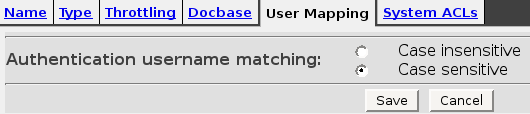
\includegraphics[width=300pt]{Docu-edit-authority-tab5}

\begin{itemize}

\item \textbf{Authentication username matching:} This option sets case
sensitivity for usernames.

\end{itemize}


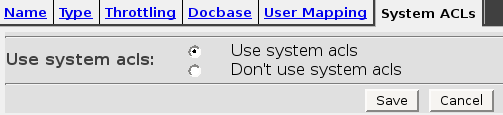
\includegraphics[width=300pt]{Docu-edit-authority-tab6}

\begin{itemize}

\item \textbf{Use system acls:} This option sets whether the GTS
appliance will use system-defined ACLs. The Documentum system
automatically generates an ACL for every folder in a docbase. Often,
ACLs of this kind are not assigned to users or groups. If your
Documentum security configuration does not use these automatically
generated ACLs, you should disable this option. The GTS appliance will
then only consider user-defined ACLs when determining file
permissions, increasing performance.

\end{itemize}




After entering this information, you will be taken to the authority
connection status page for this authority:

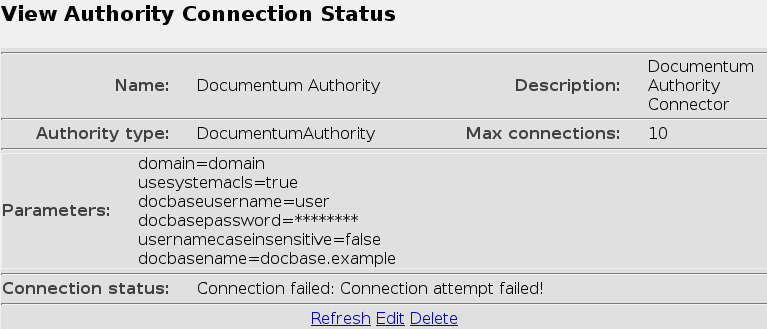
\includegraphics[width=300pt]{Docu-view-auth-conn-status}

In this example (which does not contain accurate information for any
Documentum server), the Connection Status is ``Connection failed.''
If you see this message, you most likely have incorrectly entered one
of the fields, and should click ``Edit'' to fix the data. If you have
entered everything as you intended, please inform your Documentum
administrator; you may not have been given the correct information.


\subsection{Creating Repository Connections}

Once you have created an authority connection, you need to create a
repository connection.
To do so, click ``List Repository Connections'' on the sidebar menu. Then,
when presented with the list of repository connections, click ``Add a
new connection.'' You will see the following two tabs:

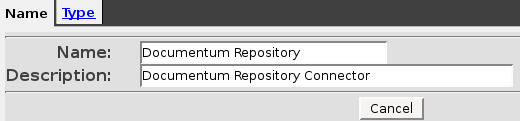
\includegraphics[width=300pt]{Docu-edit-repository-tab1}

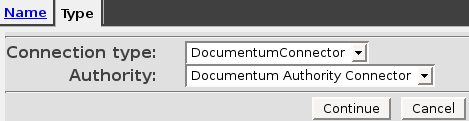
\includegraphics[width=300pt]{Docu-edit-repository-tab2}

Now you must provide a name, description, connector type, and
authority type for your new repository connection. The name should be
unique, as you will use it to select this connection later when
defining jobs. The description should explain the repository
connection to you or another administrator.  The connector type is the
type of repository from which you will get documents, in this case a
DocumentumConnector. The authority type is the type of authority from
which you will get authorization information. Typically, you will
select the Documentum authority connection that you have set up to
associate with this repository; the permissions associated with the
ingested documents will be the same as the permissions of the original
documents in the Documentum repository. If you intend to force AD ACLs
on your documents (see page \pageref{ForceACL}), then you should
select ``Standard (Kerberos)'' here.

Once you have filled in those tabs and click continue to move on to
the repository-specific options.

% Licensed to the Apache Software Foundation (ASF) under one or more
% contributor license agreements. See the NOTICE file distributed with
% this work for additional information regarding copyright ownership.
% The ASF licenses this file to You under the Apache License, Version 2.0
% (the ``License''); you may not use this file except in compliance with
% the License. You may obtain a copy of the License at
%
% http://www.apache.org/licenses/LICENSE-2.0
%
% Unless required by applicable law or agreed to in writing, software
% distributed under the License is distributed on an ``AS IS'' BASIS,
% WITHOUT WARRANTIES OR CONDITIONS OF ANY KIND, either express or implied.
% See the License for the specific language governing permissions and
% limitations under the License.

\subsubsection{Configuring a Documentum Repository}

You must fill in the following extra fields if you choose to
configure a Documentum repository connection: 

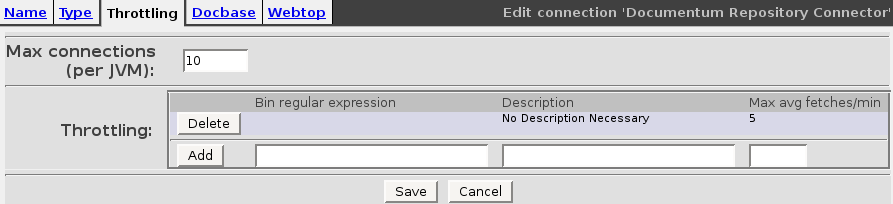
\includegraphics[width=300pt]{Docu-edit-repository-tab3}


\begin{itemize}

\item \textbf{Max connections (per JVM):} \ifCombinedConnectorGuide \label{maxrepocon} \fi Here you can set the maximum
number of connections to your repository.

The maximum number of connections per JVM is important for three
reasons.  First, the number of connections may impact the licensing on
your document server, depending on the repository. If you have a
finite number of Documentum connections available, they will be split
between the authority connector, which authorizes user access to
documents, and the repository connector, which actually downloads the
documents to the appliance. As in the case of the authority
connection, the default value of 10 connections may be a larger
portion of the available connections than you would like the GTS
appliance to use.

Second, the number of connections may impact the resources
available on the appliance. If the connector framework is slowing down
your appliance, lowering this number should help.

Third, only ten document streams can be processed by the appliance at
one time.  If you are also using other repository connectors or the
\command{ingest} command on the appliance, you should reduce this
number to prevent contention for the Ingestion interface. The
Documentum Connector will never overwhelm the interface on its own,
but when other applications are also using the ingestion interface, it
may be best to set the number of repository connections to five or
even fewer.

\item \textbf{Throttling:} Throttling allows you to limit the rate of
document ingestion based on document bins that you create with regular
expressions.

The maximum fetch rate allows you to set three things: Expression,
description, and fetches per minute. Expression allows you to provide
a regular expression to match against document bins. Each document
ingested through a connector is associated with one or more document
bins. These bins represent the servers that the connector interacts
with to obtain the document. Typically, a document will be associated
with only one document bin, representing the repository server hosting
the document. For some repository connections, documents ingested
through the connector can be hosted by different servers. In the
Documentum Connector, documents can only come from one docbase, which
you will set on the following tab. Simply leave the expression blank;
this will match any docbase you enter on the following tab.  All you
need to set is the number of document fetches per minute.  Description
is an optional field that allows you to provide a short text
description of the throttle.  Once you have set the fetch rate and
optional description, click Add.

\end{itemize}

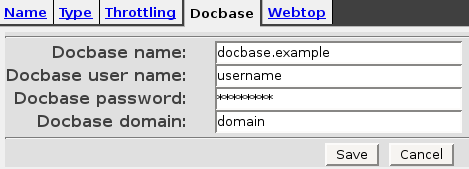
\includegraphics[width=300pt]{Docu-edit-repository-tab4}

\begin{itemize}

\item \textbf{Docbase name:} The host name of the Documentum
repository (or ``docbase'') with which you wish to connect.

\item \textbf{Docbase user name:} The user name that the GTS appliance
will use to connect to the docbase for this repository connection.
Typically, your Documentum administrator will create this account
specifically for use by the appliance. The account used by the GTS
appliance must have sufficient authority to retrieve files and their
corresponding ACLs. This may or may not be the same account used by
the GTS appliance for authority connections, depending on the security
model enforced by your Documentum administrator.

\item \textbf{Docbase password:} The password corresponding to the
username given to the GTS.

\item \textbf{Docbase domain:} The domain that the docbase is part of,
typically an Active Directory domain. This is an optional argument.

\end{itemize}

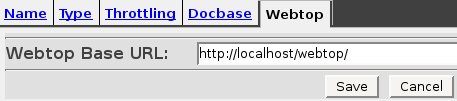
\includegraphics[width=300pt]{Docu-edit-repository-tab5}

\begin{itemize}

\item \textbf{Webtop Base URL:} The URL of the Webtop server that the
GTS appliance will use to provide MetaCarta Web Search Interface users
with document links in search results. It is recommended that you
select a Webtop server that connects to the same docbroker that the
GTS appliance uses.

\end{itemize}

After entering this information, you will be taken to the status page
for this repository connection:

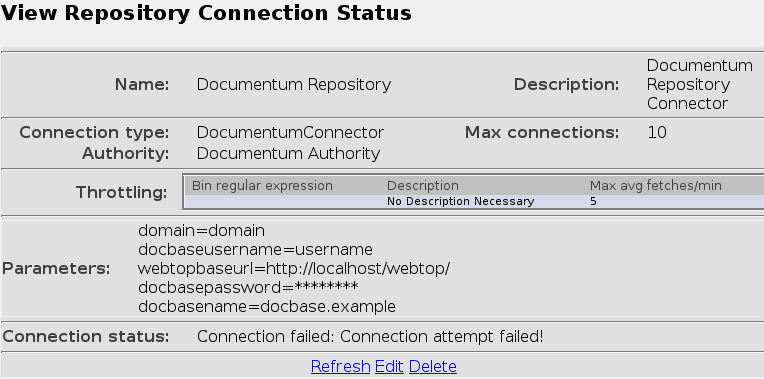
\includegraphics[width=300pt]{Docu-view-repo-conn-status}

In this example (which does not contain accurate information for any
Documentum server), the Connection Status is ``Connection failed.''
If you see this message, you most likely have incorrectly entered one
of the fields, and should click ``Edit'' to fix the data. If you have
entered everything as you intended, please inform your Documentum
administrator; you may not have been given the correct information.



\subsection{Creating and Running Jobs}

To run a job, click ``Status and Job Management'' on the sidebar menu.
You can run or edit existing jobs from this menu.

To create a new job, click ``List All Jobs'' on the sidebar menu. Then, when
presented with the list of current jobs, click ``Add a new job.'' You
will be presented with two tabs, in which you must fill in the following
information:

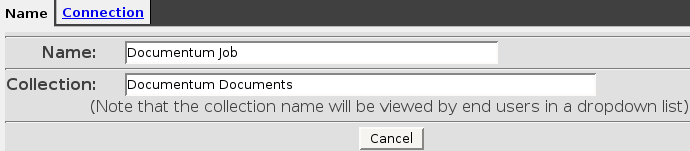
\includegraphics[width=300pt]{Docu-edit-job-tab1}

\begin{itemize}

\item \textbf{Name:} The name of the job. You will use this to identify
the job later.

\item \textbf{Collection:} The collection name metadata for all
documents in this job. End users can use this name to select the set
of documents in this job. For more information on collection name
metadata, please see the \documentref{MetaCarta GTS Administrator's
Guide}.

\end{itemize}

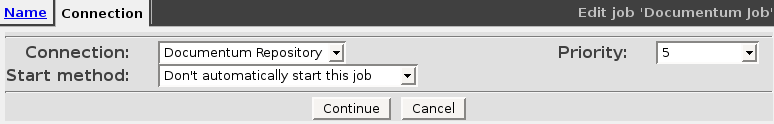
\includegraphics[width=300pt]{Docu-edit-job-tab2}

\begin{itemize}

\item \textbf{Connection:} The name of the repository connection you
wish to use for this job. You select this from the list of repository
connections you have already made. You may have more than one job use
the same repository connection, but if you have two jobs crawl the same
documents, the documents will have the metadata and collection name
associated with whatever job crawled the document most recently. This
will cause unpredictable results when searching those collections,
searching for those documents, or trying to delete those collections.
We recommend never crawling the same document in two different jobs.

\item \textbf{Start method:} Whether you want to start this job the next
time jobs are scheduled to run (``Start when schedule window starts''),
immediately after you finish defining it (``Start even inside a schedule
window''), or not at all (``Don't automatically start this job'').

\item \textbf{Priority:} From 1 (highest) to 10 (lowest), the priority
this crawl should have if it must compete for resources with other
crawls on the appliance. You should not need to change this unless you
are running more than one crawl at the same time; if you are, assign a
higher priority to the crawls whose documents you want to be processed
preferentially before documents from other jobs.

\end{itemize}

After filling in those options, click ``Continue,'' and you will be
presented with seven additional repository-specific tabs. 

% Licensed to the Apache Software Foundation (ASF) under one or more
% contributor license agreements. See the NOTICE file distributed with
% this work for additional information regarding copyright ownership.
% The ASF licenses this file to You under the Apache License, Version 2.0
% (the ``License''); you may not use this file except in compliance with
% the License. You may obtain a copy of the License at
%
% http://www.apache.org/licenses/LICENSE-2.0
%
% Unless required by applicable law or agreed to in writing, software
% distributed under the License is distributed on an ``AS IS'' BASIS,
% WITHOUT WARRANTIES OR CONDITIONS OF ANY KIND, either express or implied.
% See the License for the specific language governing permissions and
% limitations under the License.

\subsubsection{Documentum Job Options}

You must fill in the following extra fields if you choose to
configure a Documentum repository connection: 

\bigimage{Docu-edit-job-tab3}

% Licensed to the Apache Software Foundation (ASF) under one or more
% contributor license agreements. See the NOTICE file distributed with
% this work for additional information regarding copyright ownership.
% The ASF licenses this file to You under the Apache License, Version 2.0
% (the ``License''); you may not use this file except in compliance with
% the License. You may obtain a copy of the License at
%
% http://www.apache.org/licenses/LICENSE-2.0
%
% Unless required by applicable law or agreed to in writing, software
% distributed under the License is distributed on an ``AS IS'' BASIS,
% WITHOUT WARRANTIES OR CONDITIONS OF ANY KIND, either express or implied.
% See the License for the specific language governing permissions and
% limitations under the License.

\begin{itemize}
\label{scheduling}

\item \textbf{Schedule type:} Whether you want to scan every document
once or dynamically recrawl content in your repository. 

When scanning every document once, the crawler marks all documents that
have been previously crawled in this job as potentially to be deleted,
adds all seed documents to its queue and marks them as pending, processes
pending documents, marking them completed as they are ingested, and then
deleted all of the documents that were not recrawled. A document might
not be recrawled because it no longer exists, or the job specification
might have been changed to no longer include the document.

When dynamically recrawling documents, the crawler does not start by
marking all documents as potentially deletable; instead, it begins with
all of the seed documents, and continues adding to its list, periodically
re-adding the initial seed documents. If a document is removed from the
source, it will expire in the expiration interval (see below).

\item \textbf{Expiration Interval (if continuous):} The length of the
interval (in minutes) that the appliance will retain a document
crawled by this job after the document no longer appears in the
repository. After this interval, the missing document will be removed
from the appliance's index and archive. Leave the expiration interval
blank to keep missing documents indexed in GTS.

\item \textbf{Recrawl interval:} If you are dynamically recrawling
documents, how long, in minutes, the crawler should wait before
crawling documents a second time.

\item \textbf{Reseed interval:} If you are dynamically recrawling
documents, how long, in minutes, the crawler should wait before
looking for new documents to crawl. \ifMeridioGuide This connector
identifies all documents for ingestion through seeding; if the reseed
interval is infinite, the job will not ingest documents placed in the
repository during run time. (The job automatically reseeds whenever it
is started.) The default interval of 60 minutes is an appropriate
reseed rate. \fi \ifFilenetGuide This connector identifies documents
for ingestion during seeding. If you change the document inclusion
criteria, reseeding is required to identify new documents. Similarly,
documents placed in the repository while the job is running will not
be identified until the crawl is reseeded.  (The job automatically
reseeds whenever it is started.) The default interval of 60 minutes is
an appropriate reseed rate. \fi

\item \textbf{Scheduled time:} Allows you to define a time you wish
the job to run using a series of selection boxes. The first box refers
to the day of the week you wish the job to run, with an option to have
the job run any day of the week. The second box allows you to select
the start hour, with an option to start the job at any hour. The third
box allows you to specify which minute after the hour that you wish
the job to start. The fourth box allows you to specify what months of
the year you wish the job to run, with an option for the job to run
any month. The last box allows you to specify the day of the month you
wish the job to start, including any day of month.


You can scroll through each of the five boxes in this setting using
the arrow keys on your keyboard or by using the scroll bar on the
right side of the box.  If you want to select more than one value,
hold down control as you scroll and click the values that you want to
select. This allows you to define multiple windows with the same
length, for example by selecting Monday, Wednesday, and Friday at the
same time.

\item \textbf{Maximum run time:} The longest you will allow the job to
run, in minutes. For example, if you want to start a job at 2 AM but
force it to stop at 8 AM so that users have access to the repository,
you should set this value to 360 minutes. If the job is not complete by the
end time, documents that have already been found will be indexed, and
the rest of the crawl will continue at the beginning of the next
schedule interval. 

When you have defined the scheduled time and assigned a maximum run
time, click on the ``Add Scheduled Time'' button. A new schedule box
will appear below the scheduled time, allowing you to create
additional scheduled run times.

Here is a sample schedule for a job that will run every
Monday from 2 am to 6 am:

\begin{changemargin}{-.3in}{0in} 
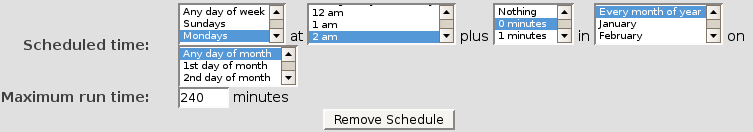
\includegraphics[width=300pt]{sample-schedule}
\end{changemargin}

If you do not have at least one scheduled time, the job will
only run when run manually (see page \pageref{ManageJobs}), and will
not automatically update the index on the appliance based on changes
to the repository.

You can remove a scheduled time by clicking the ``Remove Schedule''
button.

\end{itemize}


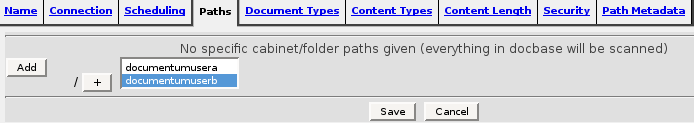
\includegraphics[width=300pt]{Docu-edit-job-tab4}

\begin{itemize}

\item \textbf{Paths:} The directory paths in your Documentum
repository from which you want your crawl to start. You can specify
one or more directory paths. If you do not specify directory paths,
the job will crawl all directories on your Documentum repository. You
can build directory paths by selecting individual directories. To
start, select the base directory of the path you wish to create, then
click the ``+'' button. A new selection box will appear with the
directories contained by that parent directory. Select a directory at
that level and click the ``+'' button. Continue building your
directory path in this fashion. When it's complete, click ``Add''. A
new selection box will appear beneath the added directory path. You
can continue to add more directory paths to your list. To remove a
directory path from the list, click the ``Delete'' button next to it.


\end{itemize}

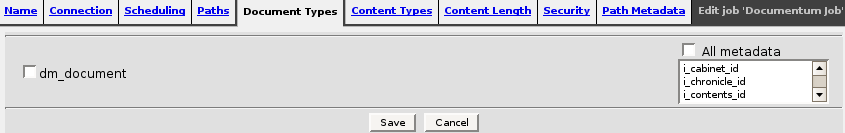
\includegraphics[width=300pt]{Docu-edit-job-tab5}

\begin{itemize}

\item \textbf{Document Types:} Select here the Documentum document
subclasses you wish to include in your job. Simply check the
subclasses you wish to include. The list of document subclasses is
generated by your Documentum repository based on existing document
subclasses.

\item \textbf{Metadata:} The Documentum repository stores various
metadata information about documents in its index.  You can select
those metadata fields here and have them sent along with the files you
index as metadata.  Each document subclass has its own selection box,
listing the metadata fields available for that particular
subclass. You can select ranges using the Shift key and make multiple
selections using the Ctrl key.  Metadata will not be geographically
parsed or used to create the index on the MetaCarta appliance;
however, with the standard MetaCarta Search APIs, you can construct
searches based specifically on this metadata. For more information on
the SOAP Search API, please see the \documentref{MetaCarta SOAP Search
API Guide}. For more information on the JSON Search API and KML Search
API, please see the \documentref{MetaCarta Guide to Web Services
Search APIs}.

\end{itemize}

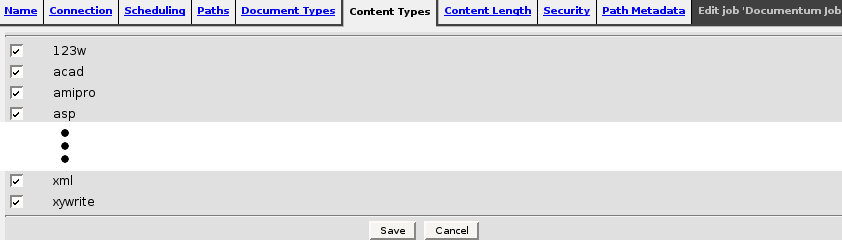
\includegraphics[width=300pt]{Docu-edit-job-tab6}

\begin{itemize}

\item \textbf{Content Types:} Here you can select the Documentum
content types you wish this job include. This list of Documentum
content types is generated by your Documentum repository based on the
content types present in the system. These content types will not
correspond directly with the filetypes supported by MetaCarta;
however, the supported filetypes provide a rough guideline for the
types of content that can be ingested.

% Licensed to the Apache Software Foundation (ASF) under one or more
% contributor license agreements. See the NOTICE file distributed with
% this work for additional information regarding copyright ownership.
% The ASF licenses this file to You under the Apache License, Version 2.0
% (the ``License''); you may not use this file except in compliance with
% the License. You may obtain a copy of the License at
%
% http://www.apache.org/licenses/LICENSE-2.0
%
% Unless required by applicable law or agreed to in writing, software
% distributed under the License is distributed on an ``AS IS'' BASIS,
% WITHOUT WARRANTIES OR CONDITIONS OF ANY KIND, either express or implied.
% See the License for the specific language governing permissions and
% limitations under the License.

MetaCarta GTS currently supports the following filetypes:

\begin{itemize}
\item ASCII Text Files with or without extensions (.txt, etc...)
\item HTML Documents (.htm, .html)
\item Adobe\circler\ Acrobat\circler\ files (.pdf)
\item Adobe PostScript\circler\ files (.ps)
\item Microsoft\circler\ Word\circler\ documents (.doc)
\item Microsoft Excel\circler\ spreadsheets (.xls)
\item Microsoft PowerPoint\circler\ presentations (.ppt)
\item Rich Text Format documents (.rtf)
\end{itemize}

\note{Documents larger than 50MB are converted to plaintext and then truncated to 50MB.} 



Some content types are easily matched to filetypes; for example the
content type \command{html} corresponds to HTML documents, and the
content type \command{pdf} corresponds to Adobe Acrobat
files. Other relationships may not be as clear. The content types
\command{msw}, \command{msw3}, \command{msw6}, \command{msw8},
\command{mwsm}, \command{mswm1}, and \command{msww} all correspond to
Microsoft Word documents, while the content type
\command{doc} corresponds to an Interleaf\circler\ 3.x or 4.x
file. Your Documentum installation includes a full list of the default
content types and their formats at
\dirpath{%DM_HOME%/install/tools/formats.csv}. See your Documentum
documentation for more details.

If documents of a given content type cannot be ingested they will not
be indexed by the appliance.

\end{itemize}

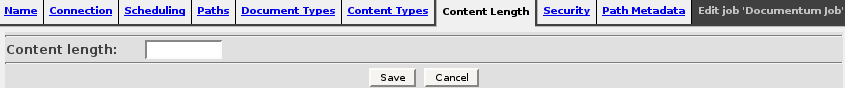
\includegraphics[width=300pt]{Docu-edit-job-tab7}

\begin{itemize}

\item \textbf{Content Length:} The maximum file size, in bytes, that
you wish this job to crawl. Files larger than this size will be
skipped. The default maximum content length is unlimited. 

\end{itemize}


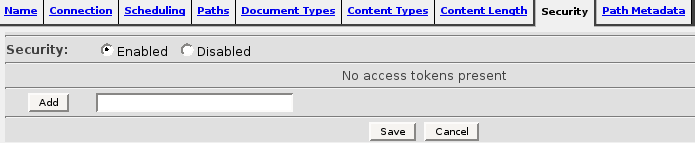
\includegraphics[width=300pt]{Docu-edit-job-tab8}

\begin{itemize}

\item \textbf{Security:} Use this option to enable or disable document
security. If you choose to enable security, user permissions will be
ingested with documents, while if you choose to disable security,
documents will be ingested without permissions.

\item \textbf{Access Tokens:} \label{ForceACL} If you wish to specify
your own ACLs for files ingested through this job, you can specify
them here. You should use this option if you selected ``Standard
(Kerberos)'' as the authority connection for your repository
connection and you are choosing to enable security. Simply enter one
or more ACL identifiers into the field and click the ``Add''
button. The ACL identifiers will appear in a list. You can continue to
add more ACL identifiers using the ``Add'' button, or remove them
using the ``Delete'' button that appears next to each ACL identifier.

\end{itemize}

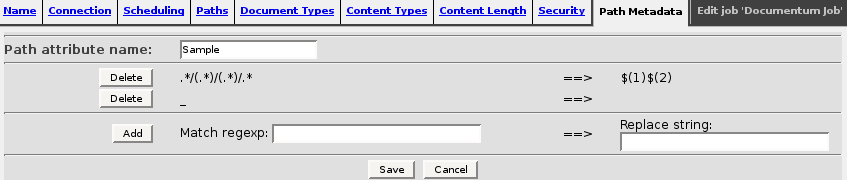
\includegraphics[width=300pt]{Docu-edit-job-tab9}

\begin{itemize}

\item \textbf{Path Attribute name:} The name for the metadata field
representing path attributes. This should be a recognizable name
distinct from any of the metadata fields already associated with any
document type being ingested. It may be useful to have the metadata
field containing path attributes have the same name across jobs.

\item \textbf{Path-value mapping:}The regular expressions and
substitutions that you want to use to collect information from the
Documentum file path. You can construct one or more regular
expressions. In the example shown, there are two expressions. The
first, \verb+.*/(.*)/(.*)/.*+ to \verb+$(1) $(2)+, would change the
directory path ``Project/Folder\_1/Folder\_2/ Filename'' into
``Folder\_1 Folder\_2.'' The second, \_ to a space, would then be
applied to turn the metadata into ``Folder 1 Folder 2.'' It is
important to allow more than one transform so that you can, if
necessary, extract text data and then parse the extracted data. The
end result of the last transform will be ingested as the value of the
metadata attribute defined previously. For more information on regular
expressions, see the note on page \pageref{regex}.

\end{itemize}


After entering this information, you will be taken to the status page
for this job:

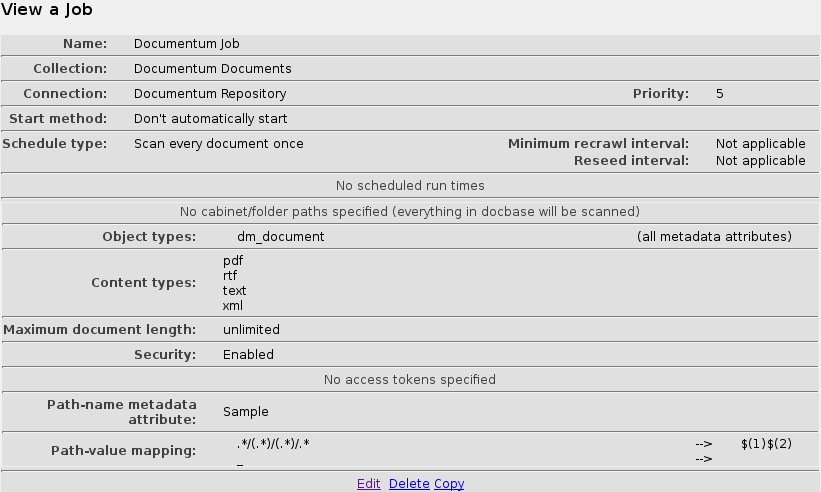
\includegraphics[width=300pt]{Docu-view-job-status}



\subsection{\label{ManageJobs}Status and Job Management}

You can then look at the status of your job by clicking ``Status and 
Job Management'' on the sidebar. You will see a list of one or more jobs
much like this one:

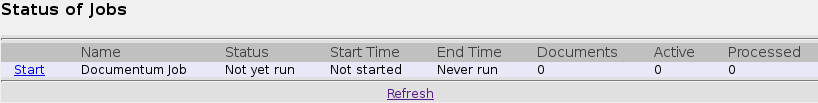
\includegraphics[width=300pt]{Docu-jobs-list}

You can start any crawl you like immediately from this interface by
clicking ``Start'' next to the name of the crawl. This interface also
allows you to see how many documents have been crawled; this information
may help you structure and plan future crawls.

\note{Refresh this page by clicking the ``Refresh'' link at the bottom
of the page, not by clicking your browser's reload button.}

\section{Reports}

The Documentum Connector interface can generate four types of reports:

\begin{itemize}

\item Simple History, which lets you list an ordered set of log events
based on chosen criteria

\item Maximum Activity, which lets you see the period of time in
which a certain event happened most often

\item Maximum Bandwith, which lets you see the period of time in
which the most bandwidth was used 

\item Result Histogram, which provides log information that would be
appropriate for constructing a histogram or other diagram

\end{itemize}

Each of these reports allows you to specify a connection, one or more
activities, a start time, an end time, an entity match, and a result code
match.  Some also allow you to specify an identifier class description
and a sliding window size. This section will show sample results for
each type of report and an explanation of the fields selected.

\subsection{Simple History}

This report was generated by selecting ``Documentum Repository Connector,'' 
clicking Continue, selecting ``fetch document,'' and clicking Go.

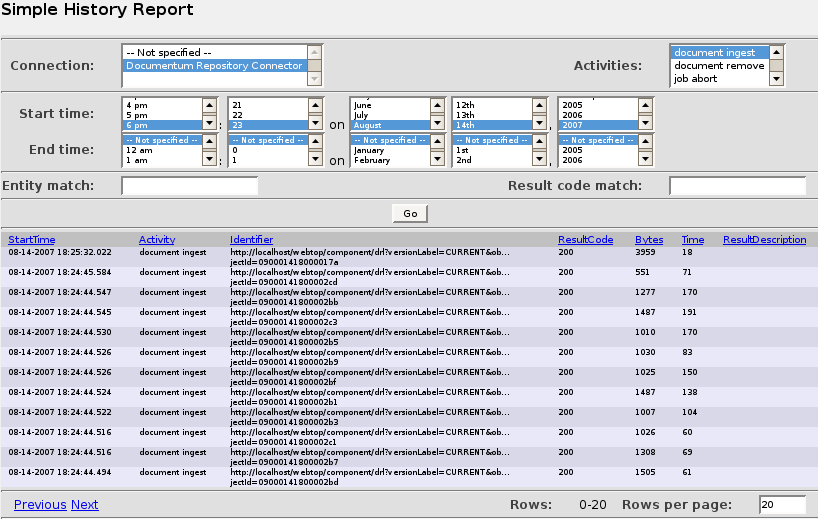
\includegraphics[width=300pt]{Docu-simple-history-report}

\begin{itemize}

\item \textbf{Connection:} The repository connection from which to generate
a report.

\item \textbf{Activities}: What crawler activities you would like to see. 
Your options are document ingest, document remove, fetch document, find 
documents, job abort, job continue, job end, job start, and job wait. 

\item \textbf{Start time}: The earliest time in the crawler logs to be
considered for this query.  Choose ``Not specified'' for any field to
start at the beginning of the crawler's logs.

\item \textbf{End time:} The latest time in the crawler logs to be
considered for this query. Choose ``Not specified'' for any field 
to end at the current time.

\item \textbf{Entity match:} A regular expression (see page
\pageref{regex}) to limit the Identifier field. If the entity match
field in the example above had been \texttt{\^{}17}, only document
fetches with Identifiers starting with 17 would be shown.

\item \textbf{Result code match:} A regular expression to limit the
ResultCode field.

\end{itemize}

You can sort the history report by any of the returned fields; to do so,
click the field names.


\subsection{Maximum Activity}

This report was generated by selecting ``Documentum Repository Connector,''
clicking Continue, selecting ``document ingest,'' changing the Identifier
class description, and clicking Go.

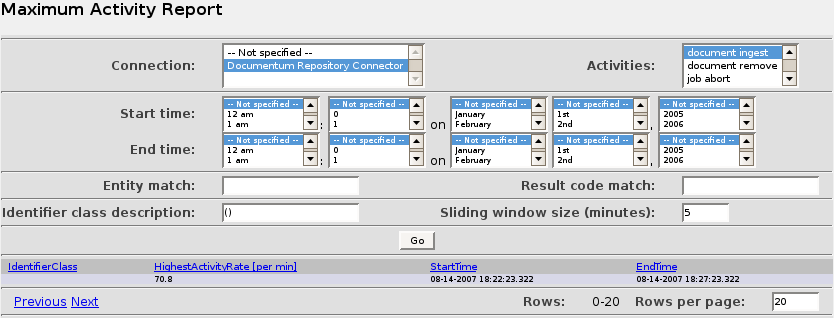
\includegraphics[width=300pt]{Docu-maximum-activity-report}

This form offers two more fields than the previous form:

\begin{itemize}

\item \textbf{Identifier class description:} A regular expression
that determines how to group identifiers together. If this were set to
\texttt{(.*)}, there would be no grouping, and so there would be only one
ingestion event per document. If this were set to \texttt{(17)},
then all documents with identifiers beginning with 17 would be grouped
together. The setting in the example, \texttt{()}, groups all
documents together. Some other possibilities:

\begin{itemize}

\item \texttt{1(.)}: (up to) Ten groups of documents whose identifier starts
with 1, labeled 0-9, grouped by the second digit of their identifier.

\item \texttt{()}: One group of documents containing all documents 
regardless of identifier.

\item \texttt{17}: One group of documents whose identifier contains
the string ``17.''

\item \texttt{\^{}17}: One group of documents whose identifier \emph{starts}
with the string ``17.''

\end{itemize}

\item \textbf{Sliding window size}: The search interval in minutes.

\end{itemize}

The report returned will have only one result per group with one or more
documents in it, if there is a clear highest activity rate, or a list of
all the results tied for highest activity rate if there are more than one.

\subsection{Maximum Bandwidth}

This report was generated by selecting ``Documentum Repository Connector,''
clicking Continue, selecting ``document ingest,'' changing the Identifier
class description, and clicking Go.

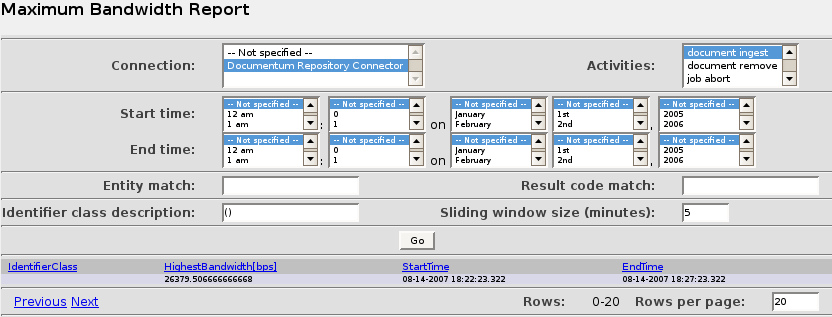
\includegraphics[width=300pt]{Docu-maximum-bandwidth-report}

This form offers the same fields as the maximum activity form, and
returns similar results; instead of tracking events per time window,
it tracks the window with the highest average bandwith usage, measured
in bytes per second. Again, the identifier class description has been
changed to a regular expression that will match all identifiers (and
thus in this case documents).

\subsection{Result Histogram}

This report was generated by selecting ``Documentum Repository Connector,''
clicking Continue, selecting ``document ingest,'' and clicking Go.

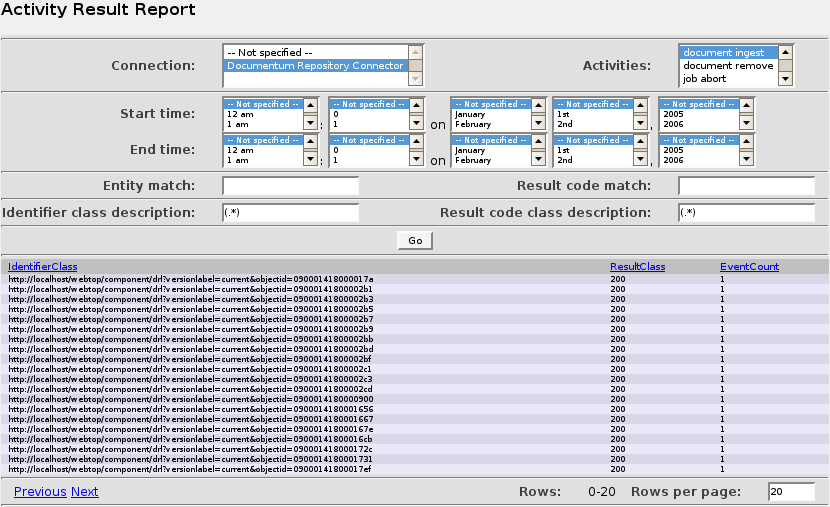
\includegraphics[width=300pt]{Docu-activity-result-report}

This form adds one new field:

\begin{itemize}

\item \textbf{Result code class description:} A regular expression that
determines how to group result classes together; like Identifier class
descriptions but for result classes.

\end{itemize}

This report does not produce an actual histogram, but provides data that
could be used to generate histograms.  

% This is a little sparse, but that's basically all this is, so.

\end{changemargin}
